\section{Validation}

The ORCA12.L46-MAL101 validation that is presented here is extracted 
from the monitoring of the experiment, available on demand on the Drakkar 
web site (contact \href{mailto:bernard.barnier@legi.grenoble-inp.fr}{bernard.barnier@legi.grenoble-inp.fr}).

\subsection{Mean state of the ocean (XXXX-XXXX)}

We present here maps of the time mean of the major ocean variables (temperature, salinity, sea surface height, barotropic transport streamfunction and meridional overturning circulation).

\begin{figure}[H]
\begin{center}
%\includegraphics[width=15cm]{FIGURES/ORCA12.L46_Tgl_0_1998-2007-MAL95.eps}
\caption{Mean Sea Surface Temperature over the period XXXX-XXXX. Colours indicate the SST in \degres C, and contour lines indicate the sea ice thickness.}
\end{center}
\end{figure}

\begin{figure}[H]
\begin{center}
%\includegraphics[width=15cm]{FIGURES/ORCA12.L46_Sgl_0_1998-2007-MAL95.eps}
\caption{Mean Sea Surface Salinity over the period XXXX-XXXX. Colours indicate the SSS, and contour lines indicate the sea ice thickness.}
\end{center}
\end{figure}

\begin{figure}[H]
\begin{center}
%\includegraphics[width=15cm]{FIGURES/ORCA12.L46_SSHGLp_0_1998-2007-MAL95.eps}
\caption{Mean Sea Surface Height over the period XXXX-XXXX. Colours indicate the SSH in meters, and contour lines indicate the sea ice thickness.}
\end{center}
\end{figure}

\begin{figure}[H]
\begin{center}
%\includegraphics[width=15cm]{FIGURES/ORCA12.L46_PSI_ATLN_1998-2007-MAL95.eps}
\caption{Mean Barotropic Streamfunction over the period XXXX-XXXX. Contours by 10 Sv, negative values are shaded.}
\end{center}
\end{figure}

\begin{figure}[H]
\begin{center}
%\includegraphics[width=10cm]{FIGURES/ORCA12.L46_OVT_glo_1998-2007-MAL95.eps}
%\includegraphics[width=10cm]{FIGURES/ORCA12.L46_OVT_atl_1998-2007-MAL95.eps}
\caption{Mean Overturning over the period XXXX-XXXX. Top: Global Ocean, bottom: Atlantic Ocean. Contours by 2 Sv.}
\end{center}
\end{figure}

\subsection{Temperature and salinity CLASS1-1}

The 10-year mean temperature difference with Levitus 2009 climatology at various depths (0m, 100m, 500m) is shown below.

\begin{figure}[H]
\begin{center}
\begin{minipage}{0.47\linewidth}
%\includegraphics[width=7cm]{FIGURES/ORCA12.L46_difTgl_k1_1998-2007-MAL95.eps}
\end{minipage}
\hfill
\begin{minipage}{0.47\linewidth}
%\includegraphics[width=7cm]{FIGURES/ORCA12.L46_difSgl_k1_1998-2007-MAL95.eps}
\end{minipage}
\begin{minipage}{0.47\linewidth}
%\includegraphics[width=7cm]{FIGURES/ORCA12.L46_difTgl_k12_1998-2007-MAL95.eps}
\end{minipage}
\hfill
\begin{minipage}{0.47\linewidth}
%\includegraphics[width=7cm]{FIGURES/ORCA12.L46_difSgl_k12_1998-2007-MAL95.eps}
\end{minipage}
\begin{minipage}{0.47\linewidth}
%\includegraphics[width=7cm]{FIGURES/ORCA12.L46_difTgl_k19_1998-2007-MAL95.eps}
\end{minipage}
\hfill
\begin{minipage}{0.47\linewidth}
%\includegraphics[width=7cm]{FIGURES/ORCA12.L46_difSgl_k19_1998-2007-MAL95.eps}
\end{minipage}
\caption{Difference between the XX-year mean temperature (left) and salinity (right) of the ORCA12.L46-MAL101 simulation 
with Levitus 2009 climatology at various depths (0m, 100m, 500m). Positive (negative) values indicate 
that the model solution is warmer or saltier (cooler or fresher) than the climatology.}
\end{center}
\end{figure}

\subsection{Heat and Freshwater surface fluxes CLASS1-4}

\begin{figure}[H]
\begin{center}
\begin{minipage}{0.47\linewidth}
%\includegraphics[width=8cm]{FIGURES/ORCA12.L46_HeatFlx_1998-2007-MAL95.eps}
\end{minipage}
\hfill
\begin{minipage}{0.47\linewidth}
%\includegraphics[width=8cm]{FIGURES/ORCA12.L46_WaterFlx_1998-2007-MAL95.eps}
\end{minipage}
\caption{ORCA12.L46-MAL101 XX-year mean net heat flux in W/m2 (left), and freshwater flux in mm/day (right).}
\end{center}
\end{figure}

\subsection{Sea-Ice CLASS1-3}

\begin{figure}[H]
\begin{center}
\begin{minipage}{0.47\linewidth}
%\includegraphics[width=8cm]{FIGURES/ORCA12.L46_N_iconc_03_1998-2007-MAL95.eps}
\end{minipage}
\hfill
\begin{minipage}{0.47\linewidth}
%\includegraphics[width=8cm]{FIGURES/ORCA12.L46_N_iconc_09_1998-2007-MAL95.eps}
\end{minipage}
\begin{minipage}{0.47\linewidth}
%\includegraphics[width=8cm]{FIGURES/ORCA12.L46_S_iconc_03_1998-2007-MAL95.eps}
\end{minipage}
\hfill
\begin{minipage}{0.47\linewidth}
%\includegraphics[width=8cm]{FIGURES/ORCA12.L46_S_iconc_09_1998-2007-MAL95.eps}
\end{minipage}
\caption{ORCA12.L46-MAL101 XX-year mean sea-ice concentration in March (left) and September (right) in the Arctic (top) and in the Antarctic (bottom).}
\end{center}
\end{figure}

\subsection{Variability}

\subsubsection{Temperature and salinity drifts}

We show here the basin averaged drifts seen in temperature and salinity during the model integration.

\begin{figure}[H]
\begin{center}
%\includegraphics[width=16cm]{FIGURES/ORCA12.L46-MAL95_tsmean.eps}
\caption{Top plots: Year-to-year variations of the world ocean average temperature and salinity over 
the integration period (XXXX-XXXX). Middle and bottom plots: Changes compared to initial condition in 
horizontally averaged temperature and salinity (vertical logarithmic depth range), left is the 
final minus initial profile, and right is the time evolution of the difference with initial condition.}
\end{center}
\end{figure}

\subsubsection{Overturning and Transport}

We show the variations during the model integration of two important climatic indexes which are the strenght of the overturning (i.e. the maximum) streamfunction in the North Atlantic, and the transport at Drake Passage.

\begin{figure}[H]
\begin{center}
%\includegraphics[width=10cm]{FIGURES/ORCA12.L46-MAL95_maxmoc-crop.eps}
\caption{Variations of the annual mean maximum overturning (Sv) in the Atlantic Ocean over the integration period (XXXX-XXXX).}
\end{center}
\end{figure}

\begin{figure}[H]
\begin{center}
%\includegraphics[width=10cm]{FIGURES/ORCA12.L46-MAL95_transports1-crop.eps}
\caption{Variations of the annual mean transport (Sv) at the Drake Passage.}
\end{center}
\end{figure}

\subsubsection{Sea-Ice variation CLASS1-3}

We show here the variation of sea-ice characteristics and especially (CLASS1-3) the sea-ice concentration in 
summer 1996 (period of maximum sea-ice coverage) and in summer 2007 (period of minimum coverage). To be compared with satellite observations.

\begin{figure}[H]
\begin{center}
\begin{minipage}{0.47\linewidth}
%\includegraphics[width=8cm]{FIGURES/ORCA12.L46_N_iconc_09_MONITOR-MAL95-1996.eps}
\end{minipage}
\hfill
\begin{minipage}{0.47\linewidth}
%\includegraphics[width=8cm]{FIGURES/ORCA12.L46_N_iconc_09_MONITOR-MAL95-2007.eps}
\end{minipage}
\caption{Sea-Ice Concentration (\%) in the Arctic in September in 1996 (left) and in 2007 (right).}
\end{center}
\end{figure}

\begin{figure}[H]
\begin{center}
%\includegraphics[width=10cm]{FIGURES/ORCA12.L46-MAL95_icetrd_min-crop.eps}
\caption{Sea-Ice Extent in September in the Arctic during the integration period (XXXX-XXXX). Blue curve is the model results and 
red curve is obtained from satellite observation. Annual means are centered on the middle of the year.}
\end{center}
\end{figure}

\subsection{El Nino}

\begin{figure}[H]
\begin{center}
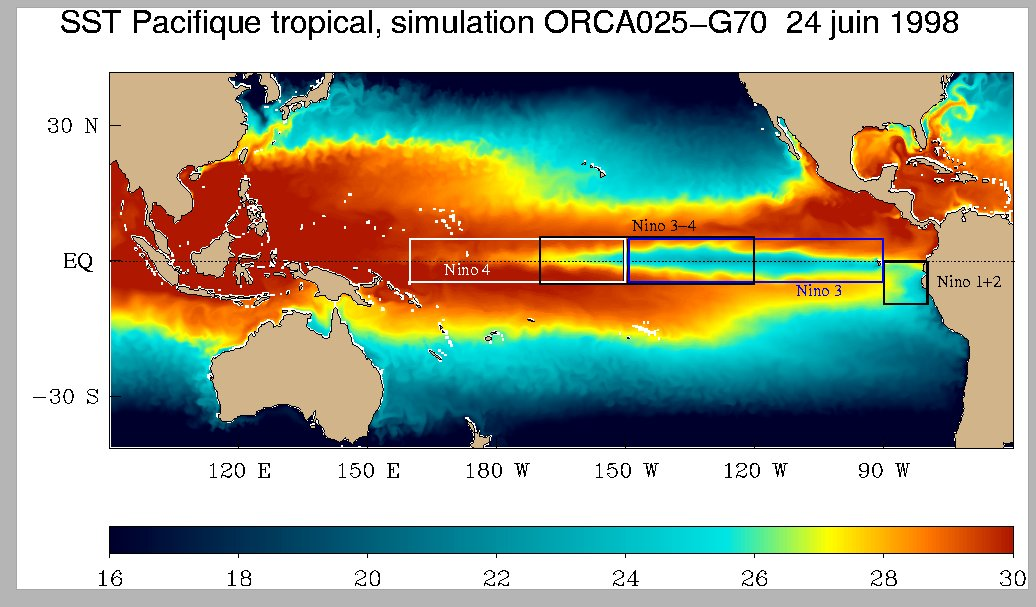
\includegraphics[width=10cm]{FIGURES/ninoboxes.eps}
\caption{Definition of the Nino boxes.}
\end{center}
\end{figure}

\begin{figure}[H]
\begin{center}
%\includegraphics[width=15cm]{FIGURES/ORCA12.L46-MAL95_nino.eps}
\caption{Monthly mean variations of the averaged temperature in el Nino boxes. Model is 
in black and observations (TOA array) are in green. Bottom plot is the Southern Oscillation 
index (monthly fluctuations in the air pressure difference between Tahiti and Darwin: sustained negative values of the SOI often indicate El Nino episodes).}
\end{center}
\end{figure}

